\documentclass[]{article}
\usepackage{lmodern}
\usepackage{amssymb,amsmath}
\usepackage{ifxetex,ifluatex}
\usepackage{fixltx2e} % provides \textsubscript
\ifnum 0\ifxetex 1\fi\ifluatex 1\fi=0 % if pdftex
  \usepackage[T1]{fontenc}
  \usepackage[utf8]{inputenc}
\else % if luatex or xelatex
  \ifxetex
    \usepackage{mathspec}
  \else
    \usepackage{fontspec}
  \fi
  \defaultfontfeatures{Ligatures=TeX,Scale=MatchLowercase}
\fi
% use upquote if available, for straight quotes in verbatim environments
\IfFileExists{upquote.sty}{\usepackage{upquote}}{}
% use microtype if available
\IfFileExists{microtype.sty}{%
\usepackage{microtype}
\UseMicrotypeSet[protrusion]{basicmath} % disable protrusion for tt fonts
}{}
\usepackage[margin=2.54cm]{geometry}
\usepackage{hyperref}
\hypersetup{unicode=true,
            pdftitle={Assignment 6: Generalized Linear Models},
            pdfauthor={Siying Chen},
            pdfborder={0 0 0},
            breaklinks=true}
\urlstyle{same}  % don't use monospace font for urls
\usepackage{color}
\usepackage{fancyvrb}
\newcommand{\VerbBar}{|}
\newcommand{\VERB}{\Verb[commandchars=\\\{\}]}
\DefineVerbatimEnvironment{Highlighting}{Verbatim}{commandchars=\\\{\}}
% Add ',fontsize=\small' for more characters per line
\usepackage{framed}
\definecolor{shadecolor}{RGB}{248,248,248}
\newenvironment{Shaded}{\begin{snugshade}}{\end{snugshade}}
\newcommand{\KeywordTok}[1]{\textcolor[rgb]{0.13,0.29,0.53}{\textbf{#1}}}
\newcommand{\DataTypeTok}[1]{\textcolor[rgb]{0.13,0.29,0.53}{#1}}
\newcommand{\DecValTok}[1]{\textcolor[rgb]{0.00,0.00,0.81}{#1}}
\newcommand{\BaseNTok}[1]{\textcolor[rgb]{0.00,0.00,0.81}{#1}}
\newcommand{\FloatTok}[1]{\textcolor[rgb]{0.00,0.00,0.81}{#1}}
\newcommand{\ConstantTok}[1]{\textcolor[rgb]{0.00,0.00,0.00}{#1}}
\newcommand{\CharTok}[1]{\textcolor[rgb]{0.31,0.60,0.02}{#1}}
\newcommand{\SpecialCharTok}[1]{\textcolor[rgb]{0.00,0.00,0.00}{#1}}
\newcommand{\StringTok}[1]{\textcolor[rgb]{0.31,0.60,0.02}{#1}}
\newcommand{\VerbatimStringTok}[1]{\textcolor[rgb]{0.31,0.60,0.02}{#1}}
\newcommand{\SpecialStringTok}[1]{\textcolor[rgb]{0.31,0.60,0.02}{#1}}
\newcommand{\ImportTok}[1]{#1}
\newcommand{\CommentTok}[1]{\textcolor[rgb]{0.56,0.35,0.01}{\textit{#1}}}
\newcommand{\DocumentationTok}[1]{\textcolor[rgb]{0.56,0.35,0.01}{\textbf{\textit{#1}}}}
\newcommand{\AnnotationTok}[1]{\textcolor[rgb]{0.56,0.35,0.01}{\textbf{\textit{#1}}}}
\newcommand{\CommentVarTok}[1]{\textcolor[rgb]{0.56,0.35,0.01}{\textbf{\textit{#1}}}}
\newcommand{\OtherTok}[1]{\textcolor[rgb]{0.56,0.35,0.01}{#1}}
\newcommand{\FunctionTok}[1]{\textcolor[rgb]{0.00,0.00,0.00}{#1}}
\newcommand{\VariableTok}[1]{\textcolor[rgb]{0.00,0.00,0.00}{#1}}
\newcommand{\ControlFlowTok}[1]{\textcolor[rgb]{0.13,0.29,0.53}{\textbf{#1}}}
\newcommand{\OperatorTok}[1]{\textcolor[rgb]{0.81,0.36,0.00}{\textbf{#1}}}
\newcommand{\BuiltInTok}[1]{#1}
\newcommand{\ExtensionTok}[1]{#1}
\newcommand{\PreprocessorTok}[1]{\textcolor[rgb]{0.56,0.35,0.01}{\textit{#1}}}
\newcommand{\AttributeTok}[1]{\textcolor[rgb]{0.77,0.63,0.00}{#1}}
\newcommand{\RegionMarkerTok}[1]{#1}
\newcommand{\InformationTok}[1]{\textcolor[rgb]{0.56,0.35,0.01}{\textbf{\textit{#1}}}}
\newcommand{\WarningTok}[1]{\textcolor[rgb]{0.56,0.35,0.01}{\textbf{\textit{#1}}}}
\newcommand{\AlertTok}[1]{\textcolor[rgb]{0.94,0.16,0.16}{#1}}
\newcommand{\ErrorTok}[1]{\textcolor[rgb]{0.64,0.00,0.00}{\textbf{#1}}}
\newcommand{\NormalTok}[1]{#1}
\usepackage{graphicx,grffile}
\makeatletter
\def\maxwidth{\ifdim\Gin@nat@width>\linewidth\linewidth\else\Gin@nat@width\fi}
\def\maxheight{\ifdim\Gin@nat@height>\textheight\textheight\else\Gin@nat@height\fi}
\makeatother
% Scale images if necessary, so that they will not overflow the page
% margins by default, and it is still possible to overwrite the defaults
% using explicit options in \includegraphics[width, height, ...]{}
\setkeys{Gin}{width=\maxwidth,height=\maxheight,keepaspectratio}
\IfFileExists{parskip.sty}{%
\usepackage{parskip}
}{% else
\setlength{\parindent}{0pt}
\setlength{\parskip}{6pt plus 2pt minus 1pt}
}
\setlength{\emergencystretch}{3em}  % prevent overfull lines
\providecommand{\tightlist}{%
  \setlength{\itemsep}{0pt}\setlength{\parskip}{0pt}}
\setcounter{secnumdepth}{0}
% Redefines (sub)paragraphs to behave more like sections
\ifx\paragraph\undefined\else
\let\oldparagraph\paragraph
\renewcommand{\paragraph}[1]{\oldparagraph{#1}\mbox{}}
\fi
\ifx\subparagraph\undefined\else
\let\oldsubparagraph\subparagraph
\renewcommand{\subparagraph}[1]{\oldsubparagraph{#1}\mbox{}}
\fi

%%% Use protect on footnotes to avoid problems with footnotes in titles
\let\rmarkdownfootnote\footnote%
\def\footnote{\protect\rmarkdownfootnote}

%%% Change title format to be more compact
\usepackage{titling}

% Create subtitle command for use in maketitle
\newcommand{\subtitle}[1]{
  \posttitle{
    \begin{center}\large#1\end{center}
    }
}

\setlength{\droptitle}{-2em}

  \title{Assignment 6: Generalized Linear Models}
    \pretitle{\vspace{\droptitle}\centering\huge}
  \posttitle{\par}
    \author{Siying Chen}
    \preauthor{\centering\large\emph}
  \postauthor{\par}
    \date{}
    \predate{}\postdate{}
  

\begin{document}
\maketitle

\subsection{OVERVIEW}\label{overview}

This exercise accompanies the lessons in Environmental Data Analytics
(ENV872L) on generalized linear models.

\subsection{Directions}\label{directions}

\begin{enumerate}
\def\labelenumi{\arabic{enumi}.}
\tightlist
\item
  Change ``Student Name'' on line 3 (above) with your name.
\item
  Use the lesson as a guide. It contains code that can be modified to
  complete the assignment.
\item
  Work through the steps, \textbf{creating code and output} that fulfill
  each instruction.
\item
  Be sure to \textbf{answer the questions} in this assignment document.
  Space for your answers is provided in this document and is indicated
  by the ``\textgreater{}'' character. If you need a second paragraph be
  sure to start the first line with ``\textgreater{}''. You should
  notice that the answer is highlighted in green by RStudio.
\item
  When you have completed the assignment, \textbf{Knit} the text and
  code into a single PDF file. You will need to have the correct
  software installed to do this (see Software Installation Guide) Press
  the \texttt{Knit} button in the RStudio scripting panel. This will
  save the PDF output in your Assignments folder.
\item
  After Knitting, please submit the completed exercise (PDF file) to the
  dropbox in Sakai. Please add your last name into the file name (e.g.,
  ``Salk\_A06\_GLMs.pdf'') prior to submission.
\end{enumerate}

The completed exercise is due on Tuesday, 26 February, 2019 before class
begins.

\subsection{Set up your session}\label{set-up-your-session}

\begin{enumerate}
\def\labelenumi{\arabic{enumi}.}
\item
  Set up your session. Upload the EPA Ecotox dataset for Neonicotinoids
  and the NTL-LTER raw data file for chemistry/physics.
\item
  Build a ggplot theme and set it as your default theme.
\end{enumerate}

\begin{Shaded}
\begin{Highlighting}[]
\CommentTok{#1}
\KeywordTok{getwd}\NormalTok{()}
\end{Highlighting}
\end{Shaded}

\begin{verbatim}
## [1] "/Users/Sylvia/Downloads/ENV872/ENV872"
\end{verbatim}

\begin{Shaded}
\begin{Highlighting}[]
\KeywordTok{library}\NormalTok{(tidyverse)}
\end{Highlighting}
\end{Shaded}

\begin{verbatim}
## -- Attaching packages ------------------------------------------------------------------------- tidyverse 1.2.1 --
\end{verbatim}

\begin{verbatim}
## v ggplot2 3.1.0     v purrr   0.2.5
## v tibble  2.0.1     v dplyr   0.7.8
## v tidyr   0.8.2     v stringr 1.3.1
## v readr   1.3.1     v forcats 0.3.0
\end{verbatim}

\begin{verbatim}
## -- Conflicts ---------------------------------------------------------------------------- tidyverse_conflicts() --
## x dplyr::filter() masks stats::filter()
## x dplyr::lag()    masks stats::lag()
\end{verbatim}

\begin{Shaded}
\begin{Highlighting}[]
\KeywordTok{library}\NormalTok{(RColorBrewer)}

\NormalTok{Ecotox <-}\StringTok{ }\KeywordTok{read.csv}\NormalTok{(}\StringTok{"./Data/Raw/ECOTOX_Neonicotinoids_Mortality_raw.csv"}\NormalTok{)}
\NormalTok{NTL_LTER.ChemPhys <-}\StringTok{ }\KeywordTok{read.csv}\NormalTok{(}\StringTok{"./Data/Raw/NTL-LTER_Lake_ChemistryPhysics_Raw.csv"}\NormalTok{)}

\CommentTok{#2}
\NormalTok{mytheme <-}\StringTok{ }\KeywordTok{theme_bw}\NormalTok{(}\DataTypeTok{base_size =} \DecValTok{14}\NormalTok{) }\OperatorTok{+}
\StringTok{  }\KeywordTok{theme}\NormalTok{(}\DataTypeTok{axis.text =} \KeywordTok{element_text}\NormalTok{(}\DataTypeTok{color =} \StringTok{"black"}\NormalTok{), }
        \DataTypeTok{legend.position =} \StringTok{"bottom"}\NormalTok{,}
        \DataTypeTok{panel.grid.major =} \KeywordTok{element_line}\NormalTok{(}\DataTypeTok{size =} \FloatTok{0.5}\NormalTok{, }\DataTypeTok{linetype =} \StringTok{'solid'}\NormalTok{), }
        \DataTypeTok{panel.grid.minor =} \KeywordTok{element_line}\NormalTok{(}\DataTypeTok{size =} \FloatTok{0.25}\NormalTok{, }\DataTypeTok{linetype =} \StringTok{'dashed'}\NormalTok{),}
        \DataTypeTok{title =} \KeywordTok{element_text}\NormalTok{(}\DataTypeTok{face =} \StringTok{"bold"}\NormalTok{))}
\KeywordTok{theme_set}\NormalTok{(mytheme)}
\end{Highlighting}
\end{Shaded}

\subsection{Neonicotinoids test}\label{neonicotinoids-test}

Research question: Were studies on various neonicotinoid chemicals
conducted in different years?

\begin{enumerate}
\def\labelenumi{\arabic{enumi}.}
\setcounter{enumi}{2}
\item
  Generate a line of code to determine how many different chemicals are
  listed in the Chemical.Name column.
\item
  Are the publication years associated with each chemical
  well-approximated by a normal distribution? Run the appropriate test
  and also generate a frequency polygon to illustrate the distribution
  of counts for each year, divided by chemical name. Bonus points if you
  can generate the results of your test from a pipe function. No need to
  make this graph pretty.
\item
  Is there equal variance among the publication years for each chemical?
  Hint: var.test is not the correct function.
\end{enumerate}

\begin{Shaded}
\begin{Highlighting}[]
\CommentTok{#3}
\KeywordTok{length}\NormalTok{(}\KeywordTok{unique}\NormalTok{(Ecotox}\OperatorTok{$}\NormalTok{Chemical.Name))}
\end{Highlighting}
\end{Shaded}

\begin{verbatim}
## [1] 9
\end{verbatim}

\begin{Shaded}
\begin{Highlighting}[]
\CommentTok{#4}
\NormalTok{Ecotox_normality <-}\StringTok{ }\NormalTok{Ecotox }\OperatorTok
\StringTok{  }\KeywordTok{group_by}\NormalTok{(Chemical.Name) }\OperatorTok
\StringTok{  }\KeywordTok{summarise}\NormalTok{(}\DataTypeTok{W =} \KeywordTok{shapiro.test}\NormalTok{(Pub..Year)}\OperatorTok{$}\NormalTok{statistic,}
            \DataTypeTok{p.value =} \KeywordTok{shapiro.test}\NormalTok{(Pub..Year)}\OperatorTok{$}\NormalTok{p.value) }
\CommentTok{# All p < 0.0001}
\CommentTok{# reject the null hypothesis and conclude that none of the data is normally distributed}

\KeywordTok{qqnorm}\NormalTok{(Ecotox}\OperatorTok{$}\NormalTok{Pub..Year); }\KeywordTok{qqline}\NormalTok{(Ecotox}\OperatorTok{$}\NormalTok{Pub..Year) }\CommentTok{# Q-Q plot confirms the previous conclusion}
\end{Highlighting}
\end{Shaded}

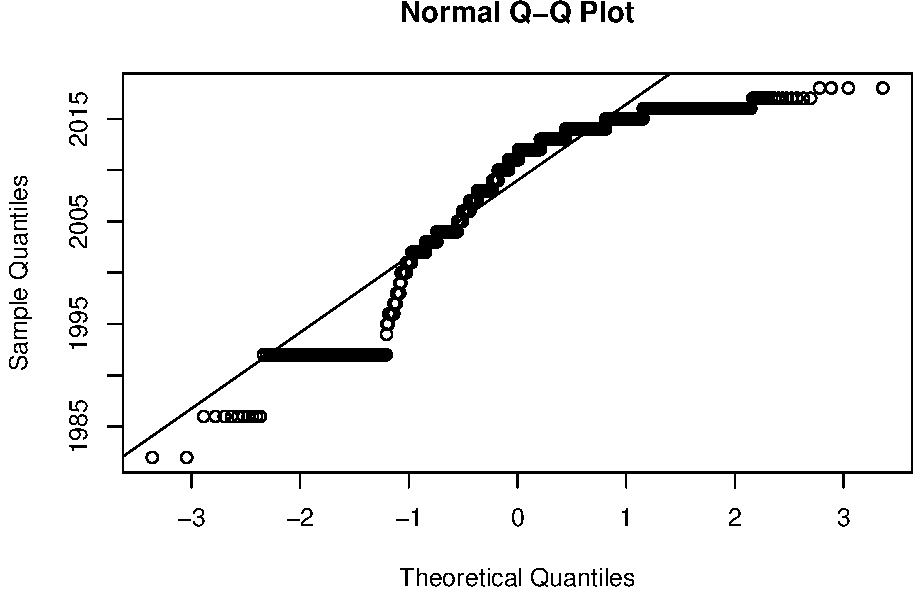
\includegraphics{A06_GLMs_files/figure-latex/unnamed-chunk-2-1.pdf}

\begin{Shaded}
\begin{Highlighting}[]
\KeywordTok{ggplot}\NormalTok{(Ecotox, }\KeywordTok{aes}\NormalTok{(}\DataTypeTok{x =}\NormalTok{ Pub..Year, }\DataTypeTok{color =}\NormalTok{ Chemical.Name)) }\OperatorTok{+}
\StringTok{  }\KeywordTok{geom_freqpoly}\NormalTok{(}\DataTypeTok{stat =} \StringTok{"count"}\NormalTok{) }\OperatorTok{+}
\StringTok{  }\KeywordTok{labs}\NormalTok{(}\DataTypeTok{x =} \StringTok{"Publication year"}\NormalTok{, }\DataTypeTok{y =} \StringTok{"Count"}\NormalTok{)}
\end{Highlighting}
\end{Shaded}

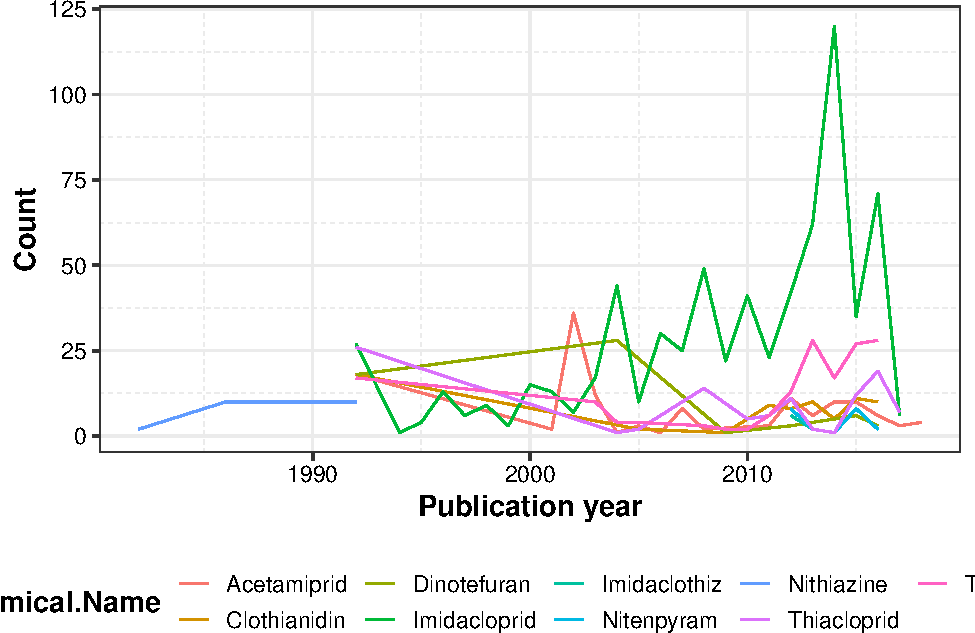
\includegraphics{A06_GLMs_files/figure-latex/unnamed-chunk-2-2.pdf}

\begin{Shaded}
\begin{Highlighting}[]
\CommentTok{#5}
\NormalTok{Ecotox_variance <-}\StringTok{ }\KeywordTok{bartlett.test}\NormalTok{(Ecotox}\OperatorTok{$}\NormalTok{Pub..Year }\OperatorTok{~}\StringTok{ }\NormalTok{Ecotox}\OperatorTok{$}\NormalTok{Chemical.Name)}
\CommentTok{# p < 0.0001}
\CommentTok{# reject the null hypothesis and conclude that not all the variances for different chemical names are the same}
\end{Highlighting}
\end{Shaded}

\begin{enumerate}
\def\labelenumi{\arabic{enumi}.}
\setcounter{enumi}{5}
\tightlist
\item
  Based on your results, which test would you choose to run to answer
  your research question?
\end{enumerate}

\begin{quote}
ANSWER: I would choose to run the one-way ANOVA test, because the there
are multiple categories in the chemical names, and a one-way ANOVA test
is similar to a two-sample t-test but for three or more groups.
\end{quote}

\begin{enumerate}
\def\labelenumi{\arabic{enumi}.}
\setcounter{enumi}{6}
\item
  Run this test below.
\item
  Generate a boxplot representing the range of publication years for
  each chemical. Adjust your graph to make it pretty.
\end{enumerate}

\begin{Shaded}
\begin{Highlighting}[]
\CommentTok{#7}
\NormalTok{Ecotox.anova <-}\StringTok{ }\KeywordTok{lm}\NormalTok{(Ecotox}\OperatorTok{$}\NormalTok{Pub..Year }\OperatorTok{~}\StringTok{ }\NormalTok{Ecotox}\OperatorTok{$}\NormalTok{Chemical.Name)}
\KeywordTok{summary}\NormalTok{(Ecotox.anova)}
\end{Highlighting}
\end{Shaded}

\begin{verbatim}
## 
## Call:
## lm(formula = Ecotox$Pub..Year ~ Ecotox$Chemical.Name)
## 
## Residuals:
##     Min      1Q  Median      3Q     Max 
## -18.366  -3.993   1.889   4.889  13.441 
## 
## Coefficients:
##                                   Estimate Std. Error  t value Pr(>|t|)
## (Intercept)                      2005.9926     0.6082 3298.222  < 2e-16
## Ecotox$Chemical.NameClothianidin    2.0479     1.0246    1.999  0.04584
## Ecotox$Chemical.NameDinotefuran    -3.4333     1.1057   -3.105  0.00194
## Ecotox$Chemical.NameImidacloprid    3.1181     0.6651    4.689 3.05e-06
## Ecotox$Chemical.NameImidaclothiz    6.4518     2.4412    2.643  0.00832
## Ecotox$Chemical.NameNitenpyram      7.7216     1.6630    4.643 3.78e-06
## Ecotox$Chemical.NameNithiazine    -17.6290     1.6299  -10.816  < 2e-16
## Ecotox$Chemical.NameThiacloprid     1.6394     0.9190    1.784  0.07467
## Ecotox$Chemical.NameThiamethoxam    4.3738     0.8261    5.295 1.40e-07
##                                     
## (Intercept)                      ***
## Ecotox$Chemical.NameClothianidin *  
## Ecotox$Chemical.NameDinotefuran  ** 
## Ecotox$Chemical.NameImidacloprid ***
## Ecotox$Chemical.NameImidaclothiz ** 
## Ecotox$Chemical.NameNitenpyram   ***
## Ecotox$Chemical.NameNithiazine   ***
## Ecotox$Chemical.NameThiacloprid  .  
## Ecotox$Chemical.NameThiamethoxam ***
## ---
## Signif. codes:  0 '***' 0.001 '**' 0.01 '*' 0.05 '.' 0.1 ' ' 1
## 
## Residual standard error: 7.093 on 1274 degrees of freedom
## Multiple R-squared:  0.1726, Adjusted R-squared:  0.1674 
## F-statistic: 33.21 on 8 and 1274 DF,  p-value: < 2.2e-16
\end{verbatim}

\begin{Shaded}
\begin{Highlighting}[]
\CommentTok{#8}
\NormalTok{Ecotox.anova.plot <-}\StringTok{ }\KeywordTok{ggplot}\NormalTok{(Ecotox, }\KeywordTok{aes}\NormalTok{(}\DataTypeTok{x =}\NormalTok{ Chemical.Name, }\DataTypeTok{y =}\NormalTok{ Pub..Year, }\DataTypeTok{fill =}\NormalTok{ Chemical.Name)) }\OperatorTok{+}
\StringTok{  }\KeywordTok{geom_boxplot}\NormalTok{(}\DataTypeTok{outlier.colour =} \StringTok{"red"}\NormalTok{) }\OperatorTok{+}
\StringTok{  }\KeywordTok{labs}\NormalTok{(}\DataTypeTok{y =} \StringTok{"Publication Year"}\NormalTok{, }\DataTypeTok{title =} \StringTok{"Studies on neonicotinoid chemicals over years"}\NormalTok{) }\OperatorTok{+}
\StringTok{  }\KeywordTok{theme}\NormalTok{(}\DataTypeTok{axis.text.x =} \KeywordTok{element_blank}\NormalTok{(), }\DataTypeTok{axis.title.x =} \KeywordTok{element_blank}\NormalTok{(), }\DataTypeTok{axis.ticks.x =} \KeywordTok{element_blank}\NormalTok{()) }\OperatorTok{+}
\StringTok{  }\KeywordTok{scale_y_discrete}\NormalTok{(}\DataTypeTok{limits =} \KeywordTok{c}\NormalTok{(}\DecValTok{1982}\NormalTok{, }\DecValTok{1990}\NormalTok{, }\DecValTok{2000}\NormalTok{, }\DecValTok{2010}\NormalTok{, }\DecValTok{2018}\NormalTok{)) }\OperatorTok{+}
\StringTok{  }\KeywordTok{scale_fill_brewer}\NormalTok{(}\DataTypeTok{palette =} \StringTok{"Set3"}\NormalTok{, }\DataTypeTok{name =} \StringTok{"Chemical Name"}\NormalTok{) }\OperatorTok{+}
\StringTok{  }\KeywordTok{guides}\NormalTok{(}\DataTypeTok{fill =} \KeywordTok{guide_legend}\NormalTok{(}\DataTypeTok{nrow =} \DecValTok{3}\NormalTok{,}\DataTypeTok{byrow =} \OtherTok{TRUE}\NormalTok{))}
\KeywordTok{print}\NormalTok{(Ecotox.anova.plot)}
\end{Highlighting}
\end{Shaded}

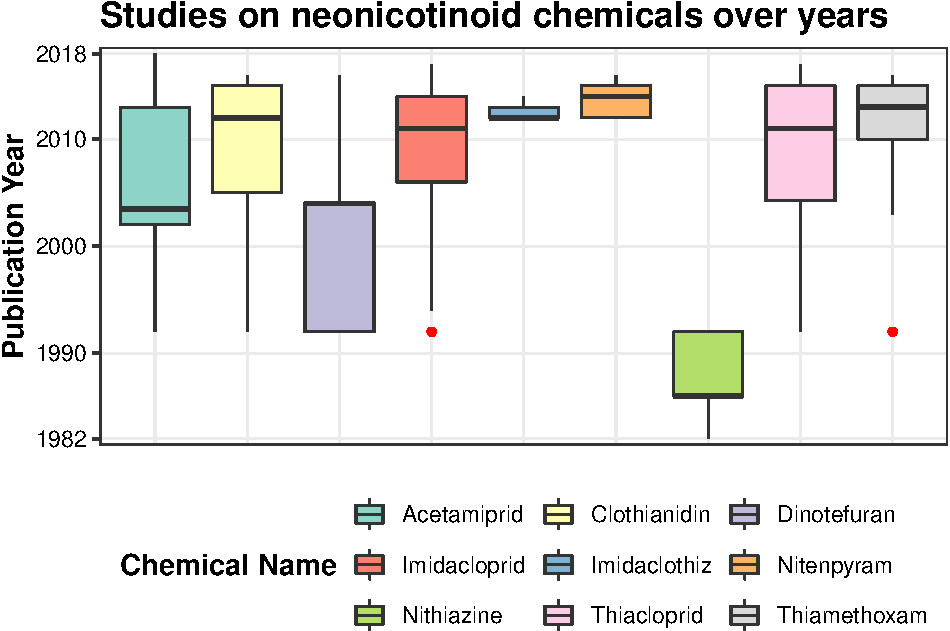
\includegraphics{A06_GLMs_files/figure-latex/unnamed-chunk-3-1.pdf}

\begin{enumerate}
\def\labelenumi{\arabic{enumi}.}
\setcounter{enumi}{8}
\tightlist
\item
  How would you summarize the conclusion of your analysis? Include a
  sentence summarizing your findings and include the results of your
  test in parentheses at the end of the sentence.
\end{enumerate}

\begin{quote}
ANSWER: The publication years of each neonicotinoid chemicals are not
normally distributed, and not all the variances for each neonicotinoid
chemicals are the same. Most of the studies on neonicotinoid chemicals
are published around 2014. However, studies on Nithiazine are mostly
published around 1988, which is also the earlieststudies on
neonicotinoid chemicals among these chosen chemicals. (one-way ANOVA; p
\textless{} 0.0001, df = 1274, F = 33.21)
\end{quote}

\subsection{NTL-LTER test}\label{ntl-lter-test}

Research question: What is the best set of predictors for lake
temperatures in July across the monitoring period at the North Temperate
Lakes LTER?

\begin{enumerate}
\def\labelenumi{\arabic{enumi}.}
\setcounter{enumi}{10}
\tightlist
\item
  Wrangle your NTL-LTER dataset with a pipe function so that it contains
  only the following criteria:
\end{enumerate}

\begin{itemize}
\tightlist
\item
  Only dates in July (hint: use the daynum column). No need to consider
  leap years.
\item
  Only the columns: lakename, year4, daynum, depth, temperature\_C
\item
  Only complete cases (i.e., remove NAs)
\end{itemize}

\begin{enumerate}
\def\labelenumi{\arabic{enumi}.}
\setcounter{enumi}{11}
\tightlist
\item
  Run an AIC to determine what set of explanatory variables (year4,
  daynum, depth) is best suited to predict temperature. Run a multiple
  regression on the recommended set of variables.
\end{enumerate}

\begin{Shaded}
\begin{Highlighting}[]
\CommentTok{#11}
\NormalTok{NTL_July <-}\StringTok{ }\NormalTok{NTL_LTER.ChemPhys }\OperatorTok
\StringTok{  }\KeywordTok{filter}\NormalTok{(daynum }\OperatorTok{>=}\StringTok{ }\DecValTok{182} \OperatorTok{&}\StringTok{ }\NormalTok{daynum }\OperatorTok{<=}\StringTok{ }\DecValTok{212}\NormalTok{) }\OperatorTok
\StringTok{  }\KeywordTok{select}\NormalTok{(lakename, year4, daynum, depth, temperature_C) }\OperatorTok
\StringTok{  }\KeywordTok{na.omit}\NormalTok{()}

\CommentTok{#12}
\NormalTok{NTL_July_AIC <-}\StringTok{ }\KeywordTok{lm}\NormalTok{(}\DataTypeTok{data =}\NormalTok{ NTL_July, temperature_C }\OperatorTok{~}\StringTok{ }\NormalTok{year4 }\OperatorTok{+}\StringTok{ }\NormalTok{daynum }\OperatorTok{+}\StringTok{ }\NormalTok{depth)}
\KeywordTok{step}\NormalTok{(NTL_July_AIC) }
\end{Highlighting}
\end{Shaded}

\begin{verbatim}
## Start:  AIC=26016.31
## temperature_C ~ year4 + daynum + depth
## 
##          Df Sum of Sq    RSS   AIC
## <none>                141118 26016
## - year4   1        80 141198 26020
## - daynum  1      1333 142450 26106
## - depth   1    403925 545042 39151
\end{verbatim}

\begin{verbatim}
## 
## Call:
## lm(formula = temperature_C ~ year4 + daynum + depth, data = NTL_July)
## 
## Coefficients:
## (Intercept)        year4       daynum        depth  
##    -6.45556      0.01013      0.04134     -1.94726
\end{verbatim}

\begin{Shaded}
\begin{Highlighting}[]
\CommentTok{# year4 has the lowest AIC, which make it the best candidate}
\CommentTok{# year4 and daynum daynum have similar AIC, which can mean they are redundant}
\CommentTok{# also daynum is already included in the initial data filter}
\CommentTok{# I would choose year and depth as explanatory variables}

\NormalTok{NTL_July_MR <-}\StringTok{ }\KeywordTok{lm}\NormalTok{(}\DataTypeTok{data =}\NormalTok{ NTL_July, temperature_C }\OperatorTok{~}\StringTok{ }\NormalTok{year4 }\OperatorTok{+}\StringTok{ }\NormalTok{depth)}
\KeywordTok{summary}\NormalTok{(NTL_July_MR)}
\end{Highlighting}
\end{Shaded}

\begin{verbatim}
## 
## Call:
## lm(formula = temperature_C ~ year4 + depth, data = NTL_July)
## 
## Residuals:
##    Min     1Q Median     3Q    Max 
## -9.541 -3.016  0.098  2.946 13.751 
## 
## Coefficients:
##              Estimate Std. Error  t value Pr(>|t|)    
## (Intercept)  1.268845   8.641177    0.147   0.8833    
## year4        0.010346   0.004323    2.393   0.0167 *  
## depth       -1.947320   0.011730 -166.013   <2e-16 ***
## ---
## Signif. codes:  0 '***' 0.001 '**' 0.01 '*' 0.05 '.' 0.1 ' ' 1
## 
## Residual standard error: 3.828 on 9719 degrees of freedom
## Multiple R-squared:  0.7393, Adjusted R-squared:  0.7392 
## F-statistic: 1.378e+04 on 2 and 9719 DF,  p-value: < 2.2e-16
\end{verbatim}

\begin{Shaded}
\begin{Highlighting}[]
\NormalTok{NTL_July_MR_plot <-}\StringTok{ }\KeywordTok{ggplot}\NormalTok{(NTL_July, }\KeywordTok{aes}\NormalTok{(}\DataTypeTok{x =}\NormalTok{ year4, }\DataTypeTok{y =}\NormalTok{ temperature_C, }\DataTypeTok{color =}\NormalTok{ depth)) }\OperatorTok{+}
\StringTok{  }\KeywordTok{geom_point}\NormalTok{(}\DataTypeTok{alpha =} \FloatTok{0.8}\NormalTok{) }\OperatorTok{+}
\StringTok{  }\KeywordTok{labs}\NormalTok{(}\DataTypeTok{x =} \StringTok{"Year"}\NormalTok{, }\DataTypeTok{y =} \StringTok{"Temperature (\textbackslash{}u00B0C)"}\NormalTok{, }\DataTypeTok{title =} \StringTok{"North Temperate Lake Temperatures in July"}\NormalTok{) }\OperatorTok{+}
\StringTok{  }\KeywordTok{scale_x_discrete}\NormalTok{(}\DataTypeTok{limits =} \KeywordTok{c}\NormalTok{(}\DecValTok{1984}\NormalTok{, }\DecValTok{1990}\NormalTok{, }\DecValTok{1995}\NormalTok{, }\DecValTok{2000}\NormalTok{, }\DecValTok{2005}\NormalTok{, }\DecValTok{2010}\NormalTok{, }\DecValTok{2016}\NormalTok{)) }\OperatorTok{+}
\StringTok{  }\KeywordTok{scale_color_distiller}\NormalTok{(}\DataTypeTok{palette =} \StringTok{"Blues"}\NormalTok{, }\DataTypeTok{direction =} \DecValTok{1}\NormalTok{, }\DataTypeTok{name =} \StringTok{"Depth (m)"}\NormalTok{) }\OperatorTok{+}
\StringTok{  }\KeywordTok{geom_smooth}\NormalTok{(}\DataTypeTok{method =} \StringTok{"lm"}\NormalTok{)}
\KeywordTok{print}\NormalTok{(NTL_July_MR_plot)}
\end{Highlighting}
\end{Shaded}

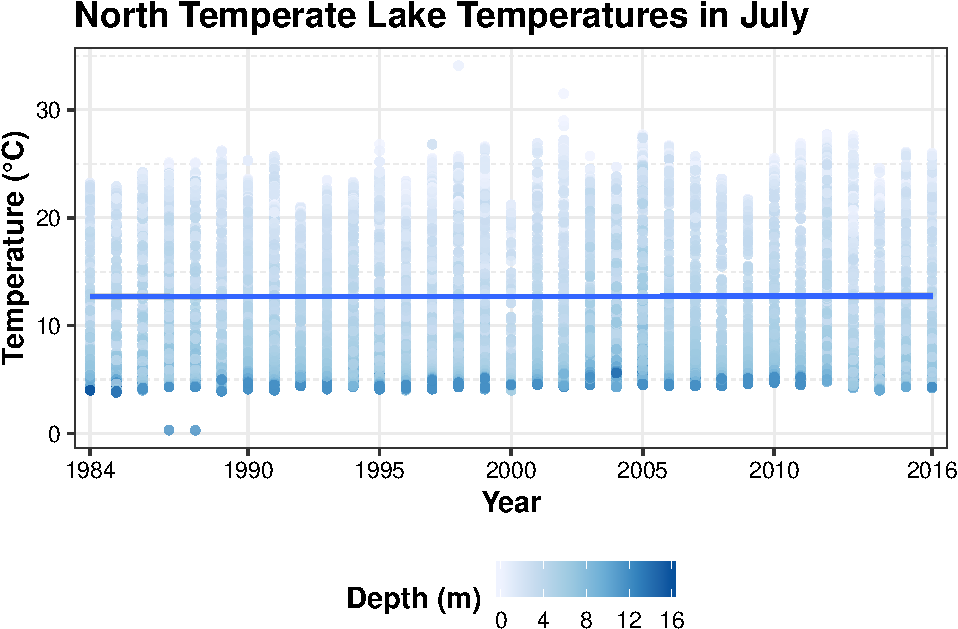
\includegraphics{A06_GLMs_files/figure-latex/unnamed-chunk-4-1.pdf}

\begin{enumerate}
\def\labelenumi{\arabic{enumi}.}
\setcounter{enumi}{12}
\tightlist
\item
  What is the final linear equation to predict temperature from your
  multiple regression? How much of the observed variance does this model
  explain?
\end{enumerate}

\begin{quote}
ANSWER: Temperature = 1.27 + 0.01(year) - 1.9(depth) + error. This model
explains about 73.92\% of the observed variance.
\end{quote}

\begin{enumerate}
\def\labelenumi{\arabic{enumi}.}
\setcounter{enumi}{13}
\tightlist
\item
  Run an interaction effects ANCOVA to predict temperature based on
  depth and lakename from the same wrangled dataset.
\end{enumerate}

\begin{Shaded}
\begin{Highlighting}[]
\CommentTok{#14}
\NormalTok{Temp_ancova.interaction <-}\StringTok{ }\KeywordTok{lm}\NormalTok{(}\DataTypeTok{data =}\NormalTok{ NTL_July, temperature_C }\OperatorTok{~}\StringTok{ }\NormalTok{lakename }\OperatorTok{*}\StringTok{ }\NormalTok{depth)}
\KeywordTok{summary}\NormalTok{(Temp_ancova.interaction)}
\end{Highlighting}
\end{Shaded}

\begin{verbatim}
## 
## Call:
## lm(formula = temperature_C ~ lakename * depth, data = NTL_July)
## 
## Residuals:
##     Min      1Q  Median      3Q     Max 
## -7.6455 -2.9133 -0.2879  2.7567 16.3606 
## 
## Coefficients:
##                                Estimate Std. Error t value Pr(>|t|)    
## (Intercept)                     22.9455     0.5861  39.147  < 2e-16 ***
## lakenameCrampton Lake            2.2173     0.6804   3.259  0.00112 ** 
## lakenameEast Long Lake          -4.3884     0.6191  -7.089 1.45e-12 ***
## lakenameHummingbird Lake        -2.4126     0.8379  -2.879  0.00399 ** 
## lakenamePaul Lake                0.6105     0.5983   1.020  0.30754    
## lakenamePeter Lake               0.2998     0.5970   0.502  0.61552    
## lakenameTuesday Lake            -2.8932     0.6060  -4.774 1.83e-06 ***
## lakenameWard Lake                2.4180     0.8434   2.867  0.00415 ** 
## lakenameWest Long Lake          -2.4663     0.6168  -3.999 6.42e-05 ***
## depth                           -2.5820     0.2411 -10.711  < 2e-16 ***
## lakenameCrampton Lake:depth      0.8058     0.2465   3.268  0.00109 ** 
## lakenameEast Long Lake:depth     0.9465     0.2433   3.891  0.00010 ***
## lakenameHummingbird Lake:depth  -0.6026     0.2919  -2.064  0.03903 *  
## lakenamePaul Lake:depth          0.4022     0.2421   1.662  0.09664 .  
## lakenamePeter Lake:depth         0.5799     0.2418   2.398  0.01649 *  
## lakenameTuesday Lake:depth       0.6605     0.2426   2.723  0.00648 ** 
## lakenameWard Lake:depth         -0.6930     0.2862  -2.421  0.01548 *  
## lakenameWest Long Lake:depth     0.8154     0.2431   3.354  0.00080 ***
## ---
## Signif. codes:  0 '***' 0.001 '**' 0.01 '*' 0.05 '.' 0.1 ' ' 1
## 
## Residual standard error: 3.471 on 9704 degrees of freedom
## Multiple R-squared:  0.7861, Adjusted R-squared:  0.7857 
## F-statistic:  2097 on 17 and 9704 DF,  p-value: < 2.2e-16
\end{verbatim}

\begin{enumerate}
\def\labelenumi{\arabic{enumi}.}
\setcounter{enumi}{14}
\tightlist
\item
  Is there an interaction between depth and lakename? How much variance
  in the temperature observations does this explain?
\end{enumerate}

\begin{quote}
ANSWER: Yes, lake temperature is associated with depth and lake name.
This model can explain about 78.57\% of the variance.
\end{quote}

\begin{enumerate}
\def\labelenumi{\arabic{enumi}.}
\setcounter{enumi}{15}
\tightlist
\item
  Create a graph that depicts temperature by depth, with a separate
  color for each lake. Add a geom\_smooth (method = ``lm'', se = FALSE)
  for each lake. Make your points 50 \% transparent. Adjust your y axis
  limits to go from 0 to 35 degrees. Clean up your graph to make it
  pretty.
\end{enumerate}

\begin{Shaded}
\begin{Highlighting}[]
\CommentTok{#16}
\NormalTok{Temp_ancova_plot <-}\StringTok{ }\KeywordTok{ggplot}\NormalTok{(NTL_LTER.ChemPhys, }\KeywordTok{aes}\NormalTok{(}\DataTypeTok{x =}\NormalTok{ depth, }\DataTypeTok{y =}\NormalTok{ temperature_C, }\DataTypeTok{color =}\NormalTok{ lakename)) }\OperatorTok{+}\StringTok{ }
\StringTok{  }\KeywordTok{geom_point}\NormalTok{(}\DataTypeTok{alpha =} \FloatTok{0.5}\NormalTok{) }\OperatorTok{+}\StringTok{ }
\StringTok{  }\KeywordTok{geom_smooth}\NormalTok{(}\DataTypeTok{method =} \StringTok{"lm"}\NormalTok{, }\DataTypeTok{se =} \OtherTok{FALSE}\NormalTok{) }\OperatorTok{+}
\StringTok{  }\KeywordTok{ylim}\NormalTok{(}\DecValTok{0}\NormalTok{,}\DecValTok{35}\NormalTok{) }\OperatorTok{+}
\StringTok{  }\KeywordTok{labs}\NormalTok{(}\DataTypeTok{x =} \StringTok{"Depth (m)"}\NormalTok{, }\DataTypeTok{y =} \StringTok{"Temperature (\textbackslash{}u00B0C)"}\NormalTok{, }\DataTypeTok{title =} \StringTok{"Lake Temperature over Depth"}\NormalTok{) }\OperatorTok{+}
\StringTok{  }\KeywordTok{scale_color_brewer}\NormalTok{(}\DataTypeTok{palette =} \StringTok{"Set1"}\NormalTok{, }\DataTypeTok{name =} \StringTok{"Lake Name"}\NormalTok{) }\OperatorTok{+}
\StringTok{  }\KeywordTok{guides}\NormalTok{(}\DataTypeTok{color =} \KeywordTok{guide_legend}\NormalTok{(}\DataTypeTok{nrow =} \DecValTok{3}\NormalTok{,}\DataTypeTok{byrow =} \OtherTok{TRUE}\NormalTok{))}
\KeywordTok{print}\NormalTok{(Temp_ancova_plot)}
\end{Highlighting}
\end{Shaded}

\begin{verbatim}
## Warning: Removed 3858 rows containing non-finite values (stat_smooth).
\end{verbatim}

\begin{verbatim}
## Warning: Removed 3858 rows containing missing values (geom_point).
\end{verbatim}

\begin{verbatim}
## Warning: Removed 126 rows containing missing values (geom_smooth).
\end{verbatim}

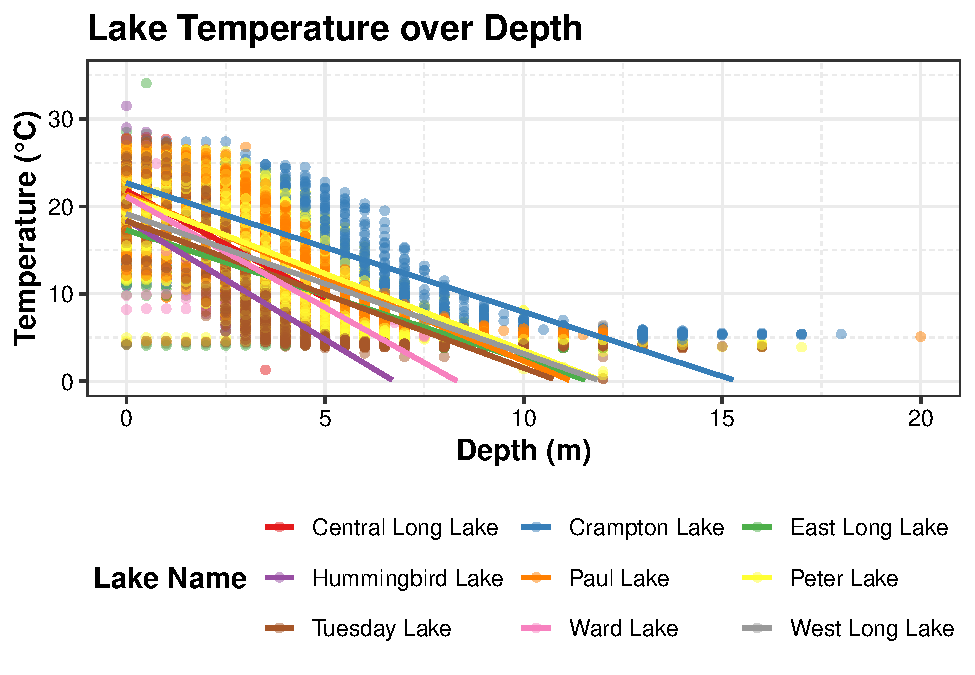
\includegraphics{A06_GLMs_files/figure-latex/unnamed-chunk-6-1.pdf}


\end{document}
